\documentclass[twoside]{book}

% Packages required by doxygen
\usepackage{fixltx2e}
\usepackage{calc}
\usepackage{doxygen}
\usepackage[export]{adjustbox} % also loads graphicx
\usepackage{graphicx}
\usepackage[utf8]{inputenc}
\usepackage{makeidx}
\usepackage{multicol}
\usepackage{multirow}
\PassOptionsToPackage{warn}{textcomp}
\usepackage{textcomp}
\usepackage[nointegrals]{wasysym}
\usepackage[table]{xcolor}

% Font selection
\usepackage[T1]{fontenc}
\usepackage[scaled=.90]{helvet}
\usepackage{courier}
\usepackage{amssymb}
\usepackage{sectsty}
\renewcommand{\familydefault}{\sfdefault}
\allsectionsfont{%
  \fontseries{bc}\selectfont%
  \color{darkgray}%
}
\renewcommand{\DoxyLabelFont}{%
  \fontseries{bc}\selectfont%
  \color{darkgray}%
}
\newcommand{\+}{\discretionary{\mbox{\scriptsize$\hookleftarrow$}}{}{}}

% Page & text layout
\usepackage{geometry}
\geometry{%
  a4paper,%
  top=2.5cm,%
  bottom=2.5cm,%
  left=2.5cm,%
  right=2.5cm%
}
\tolerance=750
\hfuzz=15pt
\hbadness=750
\setlength{\emergencystretch}{15pt}
\setlength{\parindent}{0cm}
\setlength{\parskip}{3ex plus 2ex minus 2ex}
\makeatletter
\renewcommand{\paragraph}{%
  \@startsection{paragraph}{4}{0ex}{-1.0ex}{1.0ex}{%
    \normalfont\normalsize\bfseries\SS@parafont%
  }%
}
\renewcommand{\subparagraph}{%
  \@startsection{subparagraph}{5}{0ex}{-1.0ex}{1.0ex}{%
    \normalfont\normalsize\bfseries\SS@subparafont%
  }%
}
\makeatother

% Headers & footers
\usepackage{fancyhdr}
\pagestyle{fancyplain}
\fancyhead[LE]{\fancyplain{}{\bfseries\thepage}}
\fancyhead[CE]{\fancyplain{}{}}
\fancyhead[RE]{\fancyplain{}{\bfseries\leftmark}}
\fancyhead[LO]{\fancyplain{}{\bfseries\rightmark}}
\fancyhead[CO]{\fancyplain{}{}}
\fancyhead[RO]{\fancyplain{}{\bfseries\thepage}}
\fancyfoot[LE]{\fancyplain{}{}}
\fancyfoot[CE]{\fancyplain{}{}}
\fancyfoot[RE]{\fancyplain{}{\bfseries\scriptsize Generated by Doxygen }}
\fancyfoot[LO]{\fancyplain{}{\bfseries\scriptsize Generated by Doxygen }}
\fancyfoot[CO]{\fancyplain{}{}}
\fancyfoot[RO]{\fancyplain{}{}}
\renewcommand{\footrulewidth}{0.4pt}
\renewcommand{\chaptermark}[1]{%
  \markboth{#1}{}%
}
\renewcommand{\sectionmark}[1]{%
  \markright{\thesection\ #1}%
}

% Indices & bibliography
\usepackage{natbib}
\usepackage[titles]{tocloft}
\setcounter{tocdepth}{3}
\setcounter{secnumdepth}{5}
\makeindex

% Hyperlinks (required, but should be loaded last)
\usepackage{ifpdf}
\ifpdf
  \usepackage[pdftex,pagebackref=true]{hyperref}
\else
  \usepackage[ps2pdf,pagebackref=true]{hyperref}
\fi
\hypersetup{%
  colorlinks=true,%
  linkcolor=blue,%
  citecolor=blue,%
  unicode%
}

% Custom commands
\newcommand{\clearemptydoublepage}{%
  \newpage{\pagestyle{empty}\cleardoublepage}%
}

\usepackage{caption}
\captionsetup{labelsep=space,justification=centering,font={bf},singlelinecheck=off,skip=4pt,position=top}

%===== C O N T E N T S =====

\begin{document}

% Titlepage & ToC
\hypersetup{pageanchor=false,
             bookmarksnumbered=true,
             pdfencoding=unicode
            }
\pagenumbering{alph}
\begin{titlepage}
\vspace*{7cm}
\begin{center}%
{\Large Dc\+Dc\+Converter }\\
\vspace*{1cm}
{\large Generated by Doxygen 1.8.13}\\
\end{center}
\end{titlepage}
\clearemptydoublepage
\pagenumbering{roman}
\tableofcontents
\clearemptydoublepage
\pagenumbering{arabic}
\hypersetup{pageanchor=true}

%--- Begin generated contents ---
\chapter{Mini\+Box\+D\+C\+DC}
\label{index}\hypertarget{index}{}This Python module can be used to communicate with a \href{http://www.mini-box.com/DCDC-USB-200}{\tt Mini\+Box D\+C\+D\+C-\/\+U\+S\+B-\/200} intelligent D\+C-\/\+DC converter (or other Mini\+Box converters) over a U\+SB connection. This allows for status monitoring and configuration of paramters of the module.

It uses the Python \href{https://docs.python.org/3/library/ctypes.html}{\tt {\ttfamily ctypes}} module to wrap a Windows D\+LL in pure Python and allow functions in the D\+LL to be called.

\subsection*{How to Use}

{\bfseries Note\+: this class only works with x86 (32-\/bit) versions of the Python interpreter -\/ the D\+C\+D\+C\+Usb\+Lib dll is compiled for 32-\/bit platforms only.}

{\bfseries Note 2\+: I have only tested this with Python 3.\+6.\+1 -\/ it may work with 2.\+7 or other versions.}


\begin{DoxyEnumerate}
\item Ensure you clone the \textquotesingle{}D\+LL\textquotesingle{} folder along with the Dc\+Dc\+Converter.\+py class file itself. This folder contains the D\+C\+D\+C\+Usb\+Lib.\+dll provided by Mini\+Box which packages the functions used to communicate with the module. In addition, it also contains some Microsoft Visual C++ 2005 re-\/distributables which are required by D\+C\+D\+C\+Usb\+Lib.\+dll. These can also be installed as standard system libraries by installing the \href{https://www.microsoft.com/en-us/download/details.aspx?id=3387}{\tt Microsoft Visual C++ 2005 Redistributable Package}.

The \textquotesingle{}D\+LL\textquotesingle{} folder {\bfseries must} exist in the same directory as the module file -\/ that is where the module looks when it is imported for the first time.
\item Import the module in the Python program which requires it using\+: {\ttfamily import \hyperlink{namespace_dc_dc_converter}{Dc\+Dc\+Converter}}

This loads the D\+LL into memory and makes it available for use by the class when it is initialised.
\item Initialise the class using {\ttfamily Example\+Converter\+Name = Dc\+Dc\+Converter(devcount, timer, timeout)}

Where\+:
\begin{DoxyItemize}
\item {\ttfamily devcount} is the number of the device you want to connect to -\/ use when multiple D\+C\+D\+C-\/\+U\+S\+B-\/200s are connected.
\item {\ttfamily timer} is the D\+C\+D\+C\+Usb\+Lib A\+PI refresh rate in {\bfseries seconds} -\/ ie. how often it refreses the data returned by the {\ttfamily Get\+X\+X\+X()} functions.
\item {\ttfamily timeout} is the time in seconds that should carry on trying to detect a device for, if it doesn\textquotesingle{}t detect one at first.
\end{DoxyItemize}
\end{DoxyEnumerate}

Documentation of available functions is provided within the class itself.

{\bfseries Note\+:} If the module is executed by itself (ie. as \+\_\+\+\_\+main\+\_\+\+\_\+), it will run a small test program which establishes connection with a D\+C\+D\+C-\/\+U\+S\+B-\/200 and prints out its Windows device path and firmware version. 
\chapter{Todo List}
\label{todo}
\Hypertarget{todo}

\begin{DoxyRefList}
\item[\label{todo__todo000001}%
\Hypertarget{todo__todo000001}%
Member \hyperlink{class_mini_box_d_c_d_c_1_1_dc_dc_converter_1_1_dc_dc_converter_a0340e45764fc35cdccc83da2e5e70b15}{Mini\+Box\+D\+C\+DC.Dc\+Dc\+Converter.Dc\+Dc\+Converter.Set\+Variable\+Data} (self, cnt, value)]need to test function to see what value is returned upon success/failure 
\end{DoxyRefList}
\chapter{Namespace Index}
\section{Packages}
Here are the packages with brief descriptions (if available)\+:\begin{DoxyCompactList}
\item\contentsline{section}{\hyperlink{namespace_dc_dc_converter}{Dc\+Dc\+Converter} \\*Module to communicate with D\+C-\/\+DC converters from Mini-\/\+Box.\+com }{\pageref{namespace_dc_dc_converter}}{}
\end{DoxyCompactList}

\chapter{Hierarchical Index}
\section{Class Hierarchy}
This inheritance list is sorted roughly, but not completely, alphabetically\+:\begin{DoxyCompactList}
\item object\begin{DoxyCompactList}
\item \contentsline{section}{Mini\+Box\+D\+C\+D\+C.\+Dc\+Dc\+Converter.\+Dc\+Dc\+Converter}{\pageref{class_mini_box_d_c_d_c_1_1_dc_dc_converter_1_1_dc_dc_converter}}{}
\end{DoxyCompactList}
\end{DoxyCompactList}

\chapter{Class Index}
\section{Class List}
Here are the classes, structs, unions and interfaces with brief descriptions\+:\begin{DoxyCompactList}
\item\contentsline{section}{\hyperlink{class_mini_box_d_c_d_c_1_1_dc_dc_converter_1_1_dc_dc_converter}{Mini\+Box\+D\+C\+D\+C.\+Dc\+Dc\+Converter.\+Dc\+Dc\+Converter} }{\pageref{class_mini_box_d_c_d_c_1_1_dc_dc_converter_1_1_dc_dc_converter}}{}
\end{DoxyCompactList}

\chapter{Namespace Documentation}
\hypertarget{namespace_dc_dc_converter}{}\section{Dc\+Dc\+Converter Namespace Reference}
\label{namespace_dc_dc_converter}\index{Dc\+Dc\+Converter@{Dc\+Dc\+Converter}}


Module to communicate with D\+C-\/\+DC converters from Mini-\/\+Box.\+com.  




\subsection{Detailed Description}
Module to communicate with D\+C-\/\+DC converters from Mini-\/\+Box.\+com. 

\begin{DoxyDate}{Date}
Created on 29 Jun 2017
\end{DoxyDate}
\begin{DoxyAuthor}{Author}
Jack Andrews \href{mailto:jackjackandrews2@gmail.com}{\tt jackjackandrews2@gmail.\+com} 
\end{DoxyAuthor}

\chapter{Class Documentation}
\hypertarget{class_mini_box_d_c_d_c_1_1_dc_dc_converter_1_1_dc_dc_converter}{}\section{Mini\+Box\+D\+C\+D\+C.\+Dc\+Dc\+Converter.\+Dc\+Dc\+Converter Class Reference}
\label{class_mini_box_d_c_d_c_1_1_dc_dc_converter_1_1_dc_dc_converter}\index{Mini\+Box\+D\+C\+D\+C.\+Dc\+Dc\+Converter.\+Dc\+Dc\+Converter@{Mini\+Box\+D\+C\+D\+C.\+Dc\+Dc\+Converter.\+Dc\+Dc\+Converter}}
Inheritance diagram for Mini\+Box\+D\+C\+D\+C.\+Dc\+Dc\+Converter.\+Dc\+Dc\+Converter\+:\begin{figure}[H]
\begin{center}
\leavevmode
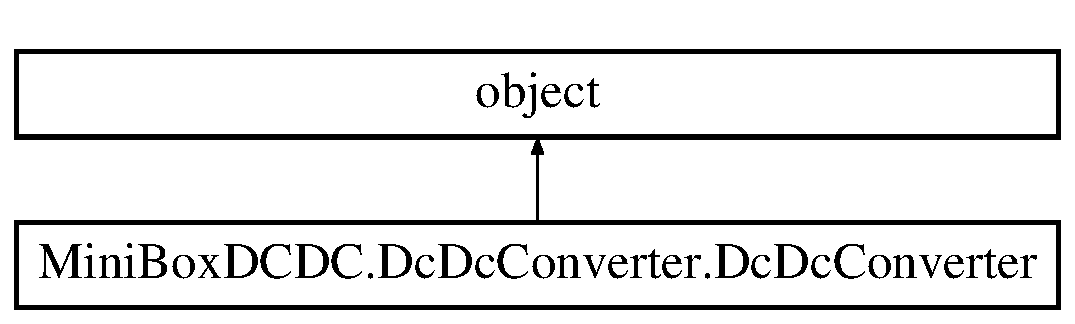
\includegraphics[height=2.000000cm]{class_mini_box_d_c_d_c_1_1_dc_dc_converter_1_1_dc_dc_converter}
\end{center}
\end{figure}
\subsection*{Public Member Functions}
\begin{DoxyCompactItemize}
\item 
def \hyperlink{class_mini_box_d_c_d_c_1_1_dc_dc_converter_1_1_dc_dc_converter_ae7aaa0ca9b46f3eecc28e3cd35d04eef}{\+\_\+\+\_\+init\+\_\+\+\_\+} (self, devcount, timer, connectiontimeout)
\begin{DoxyCompactList}\small\item\em Initialisation function for the class each time it is called. \end{DoxyCompactList}\item 
def \hyperlink{class_mini_box_d_c_d_c_1_1_dc_dc_converter_1_1_dc_dc_converter_a48fc2f6d39793c6e08b1199977f430c2}{Open\+Device} (self, timer)
\begin{DoxyCompactList}\small\item\em Opens first D\+C\+D\+C\+Usb found on U\+SB. \end{DoxyCompactList}\item 
def \hyperlink{class_mini_box_d_c_d_c_1_1_dc_dc_converter_1_1_dc_dc_converter_aa2b930875b9c91cbbe295827feb75ce6}{Open\+Device\+By\+Cnt} (self, devcount, timer)
\begin{DoxyCompactList}\small\item\em Opens devcount device (1 -\/ first device, 2 -\/ second...etc.) \end{DoxyCompactList}\item 
def \hyperlink{class_mini_box_d_c_d_c_1_1_dc_dc_converter_1_1_dc_dc_converter_a3aef4563d83abf54edc0fa5f5eaa4f62}{Get\+Device\+Path} (self, path)
\begin{DoxyCompactList}\small\item\em Get opened device path. \end{DoxyCompactList}\item 
\mbox{\Hypertarget{class_mini_box_d_c_d_c_1_1_dc_dc_converter_1_1_dc_dc_converter_a9df758198a899274cd22a4900448d1dd}\label{class_mini_box_d_c_d_c_1_1_dc_dc_converter_1_1_dc_dc_converter_a9df758198a899274cd22a4900448d1dd}} 
def \hyperlink{class_mini_box_d_c_d_c_1_1_dc_dc_converter_1_1_dc_dc_converter_a9df758198a899274cd22a4900448d1dd}{Close\+Device} (self)
\begin{DoxyCompactList}\small\item\em Close the opened D\+C\+D\+C\+Usb device. \end{DoxyCompactList}\item 
def \hyperlink{class_mini_box_d_c_d_c_1_1_dc_dc_converter_1_1_dc_dc_converter_ada9b2c23ab9374a38138078145b33936}{Get\+Connected} (self)
\begin{DoxyCompactList}\small\item\em Get connection state of the D\+C\+D\+C\+Usb. \end{DoxyCompactList}\item 
def \hyperlink{class_mini_box_d_c_d_c_1_1_dc_dc_converter_1_1_dc_dc_converter_a69f84222f6b255a67146257b09928765}{Get\+Time\+Cfg} (self)
\begin{DoxyCompactList}\small\item\em Get state variable\+: Timer Config. \end{DoxyCompactList}\item 
def \hyperlink{class_mini_box_d_c_d_c_1_1_dc_dc_converter_1_1_dc_dc_converter_a66192e46faf63db1c783a2615cb20ad8}{Get\+Voltage\+Cfg} (self)
\begin{DoxyCompactList}\small\item\em Get state variable\+: Voltage Config. \end{DoxyCompactList}\item 
def \hyperlink{class_mini_box_d_c_d_c_1_1_dc_dc_converter_1_1_dc_dc_converter_af3c0f6182a25fb1a15e5cd9558cfa117}{Get\+Mode} (self)
\begin{DoxyCompactList}\small\item\em Get state variable\+: Mode. \end{DoxyCompactList}\item 
def \hyperlink{class_mini_box_d_c_d_c_1_1_dc_dc_converter_1_1_dc_dc_converter_af0e1ad51c5ef630227e81c19010a6411}{Get\+State} (self)
\begin{DoxyCompactList}\small\item\em Get state variable\+: D\+C\+DC State. \end{DoxyCompactList}\item 
def \hyperlink{class_mini_box_d_c_d_c_1_1_dc_dc_converter_1_1_dc_dc_converter_a45d92fe89be1375296ef78e56168c472}{Get\+Vin} (self)
\begin{DoxyCompactList}\small\item\em Get state variable\+: Voltage In. \end{DoxyCompactList}\item 
def \hyperlink{class_mini_box_d_c_d_c_1_1_dc_dc_converter_1_1_dc_dc_converter_aa1bfa57870e6fd2b2ff8ff6bd0461d2c}{Get\+V\+Ign} (self)
\begin{DoxyCompactList}\small\item\em Get state variable\+: Voltage Ignition. \end{DoxyCompactList}\item 
def \hyperlink{class_mini_box_d_c_d_c_1_1_dc_dc_converter_1_1_dc_dc_converter_a1c3d70cb7dd253d4986b7cccd5a15b5e}{Get\+V\+Out} (self)
\begin{DoxyCompactList}\small\item\em Get state variable\+: Voltage Out. \end{DoxyCompactList}\item 
def \hyperlink{class_mini_box_d_c_d_c_1_1_dc_dc_converter_1_1_dc_dc_converter_a9f543016f350bf4eab819d9a23091e2f}{Get\+Enabled\+Power\+Switch} (self)
\begin{DoxyCompactList}\small\item\em Get state variable\+: Power Switch Enabled. \end{DoxyCompactList}\item 
def \hyperlink{class_mini_box_d_c_d_c_1_1_dc_dc_converter_1_1_dc_dc_converter_aac3e634377f110a6a493b45075114920}{Get\+Enabled\+Output} (self)
\begin{DoxyCompactList}\small\item\em Get state variable\+: Output Enabled. \end{DoxyCompactList}\item 
def \hyperlink{class_mini_box_d_c_d_c_1_1_dc_dc_converter_1_1_dc_dc_converter_afba56921c300608667b22030f90e8494}{Get\+Enabled\+Aux\+V\+Out} (self)
\begin{DoxyCompactList}\small\item\em Get state variable\+: Auxiliary Output Enabled. \end{DoxyCompactList}\item 
def \hyperlink{class_mini_box_d_c_d_c_1_1_dc_dc_converter_1_1_dc_dc_converter_adc2fb5f72b091473bb185ee4fe2feb8a}{Get\+Flags\+Status1} (self)
\begin{DoxyCompactList}\small\item\em Get state variable\+: Status 1 flags. \end{DoxyCompactList}\item 
def \hyperlink{class_mini_box_d_c_d_c_1_1_dc_dc_converter_1_1_dc_dc_converter_a7ec4c52f29bb150663d9346a87ed8c12}{Get\+Flags\+Status2} (self)
\begin{DoxyCompactList}\small\item\em Get state variable\+: Status 2 flags. \end{DoxyCompactList}\item 
def \hyperlink{class_mini_box_d_c_d_c_1_1_dc_dc_converter_1_1_dc_dc_converter_a0c527b680bbdcb54d903c40d2e79e06d}{Get\+Flags\+Voltage} (self)
\begin{DoxyCompactList}\small\item\em Get state variable\+: Voltage flags. \end{DoxyCompactList}\item 
def \hyperlink{class_mini_box_d_c_d_c_1_1_dc_dc_converter_1_1_dc_dc_converter_a5d9e31e7543c1eecc670a8256be37c3d}{Get\+Flags\+Timer} (self)
\begin{DoxyCompactList}\small\item\em Get state variable\+: Timer flags. \end{DoxyCompactList}\item 
def \hyperlink{class_mini_box_d_c_d_c_1_1_dc_dc_converter_1_1_dc_dc_converter_a08f751dd560392ef3e5cb7802f3f19fb}{Get\+Flash\+Pointer} (self)
\begin{DoxyCompactList}\small\item\em Get state variable\+: Flash pointer. \end{DoxyCompactList}\item 
def \hyperlink{class_mini_box_d_c_d_c_1_1_dc_dc_converter_1_1_dc_dc_converter_a0280ae59f56c09ca95d122d5e982b3ae}{Get\+Timer\+Wait} (self)
\begin{DoxyCompactList}\small\item\em Get state variable\+: Wait timer. \end{DoxyCompactList}\item 
def \hyperlink{class_mini_box_d_c_d_c_1_1_dc_dc_converter_1_1_dc_dc_converter_a303bbe36b05f402030a47cf7836869fa}{Get\+Timer\+Vout} (self)
\begin{DoxyCompactList}\small\item\em Get state variable\+: Voltage Out Timer. \end{DoxyCompactList}\item 
def \hyperlink{class_mini_box_d_c_d_c_1_1_dc_dc_converter_1_1_dc_dc_converter_aaaf98416782292ed3603f8308b9aed38}{Get\+Timer\+V\+Aux} (self)
\begin{DoxyCompactList}\small\item\em Get state variable\+: Voltage Auxiliary Timer. \end{DoxyCompactList}\item 
def \hyperlink{class_mini_box_d_c_d_c_1_1_dc_dc_converter_1_1_dc_dc_converter_a1562693daf77dc071a51d0fecd63131f}{Get\+Timer\+Pw\+Switch} (self)
\begin{DoxyCompactList}\small\item\em Get state variable\+: Power Switch Timer. \end{DoxyCompactList}\item 
def \hyperlink{class_mini_box_d_c_d_c_1_1_dc_dc_converter_1_1_dc_dc_converter_a61f1f2866b03a91566a8501251648ec7}{Get\+Timer\+Off\+Delay} (self)
\begin{DoxyCompactList}\small\item\em Get state variable\+: Off Delay Timer. \end{DoxyCompactList}\item 
def \hyperlink{class_mini_box_d_c_d_c_1_1_dc_dc_converter_1_1_dc_dc_converter_a47ac15981426ea0c5c4e8076030c043b}{Get\+Timer\+Hard\+Off} (self)
\begin{DoxyCompactList}\small\item\em Get state variable\+: Hard Off Timer. \end{DoxyCompactList}\item 
def \hyperlink{class_mini_box_d_c_d_c_1_1_dc_dc_converter_1_1_dc_dc_converter_a7422de9c9cfe5e42f5f290cbaf679f1d}{Get\+Version\+Major} (self)
\begin{DoxyCompactList}\small\item\em Get firmware version major number. \end{DoxyCompactList}\item 
def \hyperlink{class_mini_box_d_c_d_c_1_1_dc_dc_converter_1_1_dc_dc_converter_a8a8a1fdf62c9444ef7a805eafe662618}{Get\+Version\+Minor} (self)
\begin{DoxyCompactList}\small\item\em Get firmware version minor number. \end{DoxyCompactList}\item 
def \hyperlink{class_mini_box_d_c_d_c_1_1_dc_dc_converter_1_1_dc_dc_converter_a845dea85bbf256c0845cf9c499bf64d0}{Get\+Version} (self)
\begin{DoxyCompactList}\small\item\em Get firmware version (major and minor) \end{DoxyCompactList}\item 
def \hyperlink{class_mini_box_d_c_d_c_1_1_dc_dc_converter_1_1_dc_dc_converter_a0a72410596910b622eeb87b1c7aea13d}{Set\+Enabled\+Aux\+V\+Out} (self, on)
\begin{DoxyCompactList}\small\item\em Set Auxiliary Output Enable. \end{DoxyCompactList}\item 
def \hyperlink{class_mini_box_d_c_d_c_1_1_dc_dc_converter_1_1_dc_dc_converter_aec58033ac3f2a394db279b07f23168da}{Set\+Enabled\+Power\+Switch} (self, on)
\begin{DoxyCompactList}\small\item\em Set Power Switch Enable. \end{DoxyCompactList}\item 
def \hyperlink{class_mini_box_d_c_d_c_1_1_dc_dc_converter_1_1_dc_dc_converter_afde90abeae3789288591b9eeca7b26a4}{Set\+Enabled\+Output} (self, on)
\begin{DoxyCompactList}\small\item\em Set Output Enable. \end{DoxyCompactList}\item 
def \hyperlink{class_mini_box_d_c_d_c_1_1_dc_dc_converter_1_1_dc_dc_converter_a2f9ebed6d9f31e44b7bf0a6cbd8ed495}{Inc\+Dec\+V\+Out\+Volatile} (self, inc)
\begin{DoxyCompactList}\small\item\em Increase or decrease V\+Out. \end{DoxyCompactList}\item 
def \hyperlink{class_mini_box_d_c_d_c_1_1_dc_dc_converter_1_1_dc_dc_converter_a7a8cdc0b6dd49950e9ebea4e51f72a6d}{Set\+V\+Out\+Volatile} (self, vout)
\begin{DoxyCompactList}\small\item\em Set V\+Out. \end{DoxyCompactList}\item 
def \hyperlink{class_mini_box_d_c_d_c_1_1_dc_dc_converter_1_1_dc_dc_converter_af857153e7845961b8f6a3c2f9456fc42}{Load\+Flash\+Values} (self)
\begin{DoxyCompactList}\small\item\em Start loading flash values. \end{DoxyCompactList}\item 
def \hyperlink{class_mini_box_d_c_d_c_1_1_dc_dc_converter_1_1_dc_dc_converter_a914909cd3e115e6cb503f8af8250be16}{Get\+Load\+State} (self)
\begin{DoxyCompactList}\small\item\em Get loading state of flash variables. \end{DoxyCompactList}\item 
def \hyperlink{class_mini_box_d_c_d_c_1_1_dc_dc_converter_1_1_dc_dc_converter_a8aadbb6b3b47f9e2eadee5dd063f1bbf}{Get\+Max\+Variable\+Cnt} (self)
\begin{DoxyCompactList}\small\item\em Get maximum count of variables in D\+C\+D\+C\+Usb. \end{DoxyCompactList}\item 
def \hyperlink{class_mini_box_d_c_d_c_1_1_dc_dc_converter_1_1_dc_dc_converter_acbdbf705f32cdf20fc3da544241de325}{Get\+Variable\+Data} (self, cnt, name, value, unit, comment)
\begin{DoxyCompactList}\small\item\em Get the data related to a variable. \end{DoxyCompactList}\item 
def \hyperlink{class_mini_box_d_c_d_c_1_1_dc_dc_converter_1_1_dc_dc_converter_a0340e45764fc35cdccc83da2e5e70b15}{Set\+Variable\+Data} (self, cnt, value)
\begin{DoxyCompactList}\small\item\em Set one data value in PC copy of D\+C\+D\+C\+Usb Variables. \end{DoxyCompactList}\item 
def \hyperlink{class_mini_box_d_c_d_c_1_1_dc_dc_converter_1_1_dc_dc_converter_adedbbe0014ebc27f0c5dc07a3bdddeff}{Save\+Flash\+Values} (self)
\begin{DoxyCompactList}\small\item\em Save the full flash to D\+C\+D\+C\+Usb. \end{DoxyCompactList}\end{DoxyCompactItemize}


\subsection{Constructor \& Destructor Documentation}
\mbox{\Hypertarget{class_mini_box_d_c_d_c_1_1_dc_dc_converter_1_1_dc_dc_converter_ae7aaa0ca9b46f3eecc28e3cd35d04eef}\label{class_mini_box_d_c_d_c_1_1_dc_dc_converter_1_1_dc_dc_converter_ae7aaa0ca9b46f3eecc28e3cd35d04eef}} 
\index{Mini\+Box\+D\+C\+D\+C\+::\+Dc\+Dc\+Converter\+::\+Dc\+Dc\+Converter@{Mini\+Box\+D\+C\+D\+C\+::\+Dc\+Dc\+Converter\+::\+Dc\+Dc\+Converter}!\+\_\+\+\_\+init\+\_\+\+\_\+@{\+\_\+\+\_\+init\+\_\+\+\_\+}}
\index{\+\_\+\+\_\+init\+\_\+\+\_\+@{\+\_\+\+\_\+init\+\_\+\+\_\+}!Mini\+Box\+D\+C\+D\+C\+::\+Dc\+Dc\+Converter\+::\+Dc\+Dc\+Converter@{Mini\+Box\+D\+C\+D\+C\+::\+Dc\+Dc\+Converter\+::\+Dc\+Dc\+Converter}}
\subsubsection{\texorpdfstring{\+\_\+\+\_\+init\+\_\+\+\_\+()}{\_\_init\_\_()}}
{\footnotesize\ttfamily def Mini\+Box\+D\+C\+D\+C.\+Dc\+Dc\+Converter.\+Dc\+Dc\+Converter.\+\_\+\+\_\+init\+\_\+\+\_\+ (\begin{DoxyParamCaption}\item[{}]{self,  }\item[{}]{devcount,  }\item[{}]{timer,  }\item[{}]{connectiontimeout }\end{DoxyParamCaption})}



Initialisation function for the class each time it is called. 


\begin{DoxyParams}{Parameters}
{\em devcount} & number of device to be opened \\
\hline
{\em timer} & period (seconds) for A\+PI data refresh rate \\
\hline
{\em connectiontimeout} & how long to keep trying to connect if connection fails first time (seconds)\\
\hline
\end{DoxyParams}
\begin{DoxySeeAlso}{See also}
\hyperlink{class_mini_box_d_c_d_c_1_1_dc_dc_converter_1_1_dc_dc_converter_a48fc2f6d39793c6e08b1199977f430c2}{Open\+Device} 

\hyperlink{class_mini_box_d_c_d_c_1_1_dc_dc_converter_1_1_dc_dc_converter_aa2b930875b9c91cbbe295827feb75ce6}{Open\+Device\+By\+Cnt} 
\end{DoxySeeAlso}


\subsection{Member Function Documentation}
\mbox{\Hypertarget{class_mini_box_d_c_d_c_1_1_dc_dc_converter_1_1_dc_dc_converter_ada9b2c23ab9374a38138078145b33936}\label{class_mini_box_d_c_d_c_1_1_dc_dc_converter_1_1_dc_dc_converter_ada9b2c23ab9374a38138078145b33936}} 
\index{Mini\+Box\+D\+C\+D\+C\+::\+Dc\+Dc\+Converter\+::\+Dc\+Dc\+Converter@{Mini\+Box\+D\+C\+D\+C\+::\+Dc\+Dc\+Converter\+::\+Dc\+Dc\+Converter}!Get\+Connected@{Get\+Connected}}
\index{Get\+Connected@{Get\+Connected}!Mini\+Box\+D\+C\+D\+C\+::\+Dc\+Dc\+Converter\+::\+Dc\+Dc\+Converter@{Mini\+Box\+D\+C\+D\+C\+::\+Dc\+Dc\+Converter\+::\+Dc\+Dc\+Converter}}
\subsubsection{\texorpdfstring{Get\+Connected()}{GetConnected()}}
{\footnotesize\ttfamily def Mini\+Box\+D\+C\+D\+C.\+Dc\+Dc\+Converter.\+Dc\+Dc\+Converter.\+Get\+Connected (\begin{DoxyParamCaption}\item[{}]{self }\end{DoxyParamCaption})}



Get connection state of the D\+C\+D\+C\+Usb. 

\begin{DoxyReturn}{Returns}
1 on connected state, 0 on not connected 
\end{DoxyReturn}
\mbox{\Hypertarget{class_mini_box_d_c_d_c_1_1_dc_dc_converter_1_1_dc_dc_converter_a3aef4563d83abf54edc0fa5f5eaa4f62}\label{class_mini_box_d_c_d_c_1_1_dc_dc_converter_1_1_dc_dc_converter_a3aef4563d83abf54edc0fa5f5eaa4f62}} 
\index{Mini\+Box\+D\+C\+D\+C\+::\+Dc\+Dc\+Converter\+::\+Dc\+Dc\+Converter@{Mini\+Box\+D\+C\+D\+C\+::\+Dc\+Dc\+Converter\+::\+Dc\+Dc\+Converter}!Get\+Device\+Path@{Get\+Device\+Path}}
\index{Get\+Device\+Path@{Get\+Device\+Path}!Mini\+Box\+D\+C\+D\+C\+::\+Dc\+Dc\+Converter\+::\+Dc\+Dc\+Converter@{Mini\+Box\+D\+C\+D\+C\+::\+Dc\+Dc\+Converter\+::\+Dc\+Dc\+Converter}}
\subsubsection{\texorpdfstring{Get\+Device\+Path()}{GetDevicePath()}}
{\footnotesize\ttfamily def Mini\+Box\+D\+C\+D\+C.\+Dc\+Dc\+Converter.\+Dc\+Dc\+Converter.\+Get\+Device\+Path (\begin{DoxyParamCaption}\item[{}]{self,  }\item[{}]{path }\end{DoxyParamCaption})}



Get opened device path. 

Pointer to char can be created using standard Python method \begin{DoxyVerb}dev_path = create_string_buffer(init, size)
\end{DoxyVerb}


Then pass in dev\+\_\+path to the method.

Path can be decoded using standard Python method \begin{DoxyVerb}dev_path.value.decode('UTF-8')
\end{DoxyVerb}


Assuming U\+T\+F-\/8 encoding.


\begin{DoxyParams}{Parameters}
{\em path} & c-\/type pointer to char, minimum length 1024 \\
\hline
\end{DoxyParams}
\mbox{\Hypertarget{class_mini_box_d_c_d_c_1_1_dc_dc_converter_1_1_dc_dc_converter_afba56921c300608667b22030f90e8494}\label{class_mini_box_d_c_d_c_1_1_dc_dc_converter_1_1_dc_dc_converter_afba56921c300608667b22030f90e8494}} 
\index{Mini\+Box\+D\+C\+D\+C\+::\+Dc\+Dc\+Converter\+::\+Dc\+Dc\+Converter@{Mini\+Box\+D\+C\+D\+C\+::\+Dc\+Dc\+Converter\+::\+Dc\+Dc\+Converter}!Get\+Enabled\+Aux\+V\+Out@{Get\+Enabled\+Aux\+V\+Out}}
\index{Get\+Enabled\+Aux\+V\+Out@{Get\+Enabled\+Aux\+V\+Out}!Mini\+Box\+D\+C\+D\+C\+::\+Dc\+Dc\+Converter\+::\+Dc\+Dc\+Converter@{Mini\+Box\+D\+C\+D\+C\+::\+Dc\+Dc\+Converter\+::\+Dc\+Dc\+Converter}}
\subsubsection{\texorpdfstring{Get\+Enabled\+Aux\+V\+Out()}{GetEnabledAuxVOut()}}
{\footnotesize\ttfamily def Mini\+Box\+D\+C\+D\+C.\+Dc\+Dc\+Converter.\+Dc\+Dc\+Converter.\+Get\+Enabled\+Aux\+V\+Out (\begin{DoxyParamCaption}\item[{}]{self }\end{DoxyParamCaption})}



Get state variable\+: Auxiliary Output Enabled. 

\begin{DoxyReturn}{Returns}
State variable\+: Auxiliary Output Enabled 
\end{DoxyReturn}
\mbox{\Hypertarget{class_mini_box_d_c_d_c_1_1_dc_dc_converter_1_1_dc_dc_converter_aac3e634377f110a6a493b45075114920}\label{class_mini_box_d_c_d_c_1_1_dc_dc_converter_1_1_dc_dc_converter_aac3e634377f110a6a493b45075114920}} 
\index{Mini\+Box\+D\+C\+D\+C\+::\+Dc\+Dc\+Converter\+::\+Dc\+Dc\+Converter@{Mini\+Box\+D\+C\+D\+C\+::\+Dc\+Dc\+Converter\+::\+Dc\+Dc\+Converter}!Get\+Enabled\+Output@{Get\+Enabled\+Output}}
\index{Get\+Enabled\+Output@{Get\+Enabled\+Output}!Mini\+Box\+D\+C\+D\+C\+::\+Dc\+Dc\+Converter\+::\+Dc\+Dc\+Converter@{Mini\+Box\+D\+C\+D\+C\+::\+Dc\+Dc\+Converter\+::\+Dc\+Dc\+Converter}}
\subsubsection{\texorpdfstring{Get\+Enabled\+Output()}{GetEnabledOutput()}}
{\footnotesize\ttfamily def Mini\+Box\+D\+C\+D\+C.\+Dc\+Dc\+Converter.\+Dc\+Dc\+Converter.\+Get\+Enabled\+Output (\begin{DoxyParamCaption}\item[{}]{self }\end{DoxyParamCaption})}



Get state variable\+: Output Enabled. 

\begin{DoxyReturn}{Returns}
State variable\+: Output Enabled 
\end{DoxyReturn}
\mbox{\Hypertarget{class_mini_box_d_c_d_c_1_1_dc_dc_converter_1_1_dc_dc_converter_a9f543016f350bf4eab819d9a23091e2f}\label{class_mini_box_d_c_d_c_1_1_dc_dc_converter_1_1_dc_dc_converter_a9f543016f350bf4eab819d9a23091e2f}} 
\index{Mini\+Box\+D\+C\+D\+C\+::\+Dc\+Dc\+Converter\+::\+Dc\+Dc\+Converter@{Mini\+Box\+D\+C\+D\+C\+::\+Dc\+Dc\+Converter\+::\+Dc\+Dc\+Converter}!Get\+Enabled\+Power\+Switch@{Get\+Enabled\+Power\+Switch}}
\index{Get\+Enabled\+Power\+Switch@{Get\+Enabled\+Power\+Switch}!Mini\+Box\+D\+C\+D\+C\+::\+Dc\+Dc\+Converter\+::\+Dc\+Dc\+Converter@{Mini\+Box\+D\+C\+D\+C\+::\+Dc\+Dc\+Converter\+::\+Dc\+Dc\+Converter}}
\subsubsection{\texorpdfstring{Get\+Enabled\+Power\+Switch()}{GetEnabledPowerSwitch()}}
{\footnotesize\ttfamily def Mini\+Box\+D\+C\+D\+C.\+Dc\+Dc\+Converter.\+Dc\+Dc\+Converter.\+Get\+Enabled\+Power\+Switch (\begin{DoxyParamCaption}\item[{}]{self }\end{DoxyParamCaption})}



Get state variable\+: Power Switch Enabled. 

\begin{DoxyReturn}{Returns}
State variable\+: Power Switch Enabled 
\end{DoxyReturn}
\mbox{\Hypertarget{class_mini_box_d_c_d_c_1_1_dc_dc_converter_1_1_dc_dc_converter_adc2fb5f72b091473bb185ee4fe2feb8a}\label{class_mini_box_d_c_d_c_1_1_dc_dc_converter_1_1_dc_dc_converter_adc2fb5f72b091473bb185ee4fe2feb8a}} 
\index{Mini\+Box\+D\+C\+D\+C\+::\+Dc\+Dc\+Converter\+::\+Dc\+Dc\+Converter@{Mini\+Box\+D\+C\+D\+C\+::\+Dc\+Dc\+Converter\+::\+Dc\+Dc\+Converter}!Get\+Flags\+Status1@{Get\+Flags\+Status1}}
\index{Get\+Flags\+Status1@{Get\+Flags\+Status1}!Mini\+Box\+D\+C\+D\+C\+::\+Dc\+Dc\+Converter\+::\+Dc\+Dc\+Converter@{Mini\+Box\+D\+C\+D\+C\+::\+Dc\+Dc\+Converter\+::\+Dc\+Dc\+Converter}}
\subsubsection{\texorpdfstring{Get\+Flags\+Status1()}{GetFlagsStatus1()}}
{\footnotesize\ttfamily def Mini\+Box\+D\+C\+D\+C.\+Dc\+Dc\+Converter.\+Dc\+Dc\+Converter.\+Get\+Flags\+Status1 (\begin{DoxyParamCaption}\item[{}]{self }\end{DoxyParamCaption})}



Get state variable\+: Status 1 flags. 

\begin{DoxyReturn}{Returns}
State variable\+: Status 1 flags 
\end{DoxyReturn}
\mbox{\Hypertarget{class_mini_box_d_c_d_c_1_1_dc_dc_converter_1_1_dc_dc_converter_a7ec4c52f29bb150663d9346a87ed8c12}\label{class_mini_box_d_c_d_c_1_1_dc_dc_converter_1_1_dc_dc_converter_a7ec4c52f29bb150663d9346a87ed8c12}} 
\index{Mini\+Box\+D\+C\+D\+C\+::\+Dc\+Dc\+Converter\+::\+Dc\+Dc\+Converter@{Mini\+Box\+D\+C\+D\+C\+::\+Dc\+Dc\+Converter\+::\+Dc\+Dc\+Converter}!Get\+Flags\+Status2@{Get\+Flags\+Status2}}
\index{Get\+Flags\+Status2@{Get\+Flags\+Status2}!Mini\+Box\+D\+C\+D\+C\+::\+Dc\+Dc\+Converter\+::\+Dc\+Dc\+Converter@{Mini\+Box\+D\+C\+D\+C\+::\+Dc\+Dc\+Converter\+::\+Dc\+Dc\+Converter}}
\subsubsection{\texorpdfstring{Get\+Flags\+Status2()}{GetFlagsStatus2()}}
{\footnotesize\ttfamily def Mini\+Box\+D\+C\+D\+C.\+Dc\+Dc\+Converter.\+Dc\+Dc\+Converter.\+Get\+Flags\+Status2 (\begin{DoxyParamCaption}\item[{}]{self }\end{DoxyParamCaption})}



Get state variable\+: Status 2 flags. 

\begin{DoxyReturn}{Returns}
State variable\+: Status 2 flags 
\end{DoxyReturn}
\mbox{\Hypertarget{class_mini_box_d_c_d_c_1_1_dc_dc_converter_1_1_dc_dc_converter_a5d9e31e7543c1eecc670a8256be37c3d}\label{class_mini_box_d_c_d_c_1_1_dc_dc_converter_1_1_dc_dc_converter_a5d9e31e7543c1eecc670a8256be37c3d}} 
\index{Mini\+Box\+D\+C\+D\+C\+::\+Dc\+Dc\+Converter\+::\+Dc\+Dc\+Converter@{Mini\+Box\+D\+C\+D\+C\+::\+Dc\+Dc\+Converter\+::\+Dc\+Dc\+Converter}!Get\+Flags\+Timer@{Get\+Flags\+Timer}}
\index{Get\+Flags\+Timer@{Get\+Flags\+Timer}!Mini\+Box\+D\+C\+D\+C\+::\+Dc\+Dc\+Converter\+::\+Dc\+Dc\+Converter@{Mini\+Box\+D\+C\+D\+C\+::\+Dc\+Dc\+Converter\+::\+Dc\+Dc\+Converter}}
\subsubsection{\texorpdfstring{Get\+Flags\+Timer()}{GetFlagsTimer()}}
{\footnotesize\ttfamily def Mini\+Box\+D\+C\+D\+C.\+Dc\+Dc\+Converter.\+Dc\+Dc\+Converter.\+Get\+Flags\+Timer (\begin{DoxyParamCaption}\item[{}]{self }\end{DoxyParamCaption})}



Get state variable\+: Timer flags. 

\begin{DoxyReturn}{Returns}
State variable\+: Timer flags 
\end{DoxyReturn}
\mbox{\Hypertarget{class_mini_box_d_c_d_c_1_1_dc_dc_converter_1_1_dc_dc_converter_a0c527b680bbdcb54d903c40d2e79e06d}\label{class_mini_box_d_c_d_c_1_1_dc_dc_converter_1_1_dc_dc_converter_a0c527b680bbdcb54d903c40d2e79e06d}} 
\index{Mini\+Box\+D\+C\+D\+C\+::\+Dc\+Dc\+Converter\+::\+Dc\+Dc\+Converter@{Mini\+Box\+D\+C\+D\+C\+::\+Dc\+Dc\+Converter\+::\+Dc\+Dc\+Converter}!Get\+Flags\+Voltage@{Get\+Flags\+Voltage}}
\index{Get\+Flags\+Voltage@{Get\+Flags\+Voltage}!Mini\+Box\+D\+C\+D\+C\+::\+Dc\+Dc\+Converter\+::\+Dc\+Dc\+Converter@{Mini\+Box\+D\+C\+D\+C\+::\+Dc\+Dc\+Converter\+::\+Dc\+Dc\+Converter}}
\subsubsection{\texorpdfstring{Get\+Flags\+Voltage()}{GetFlagsVoltage()}}
{\footnotesize\ttfamily def Mini\+Box\+D\+C\+D\+C.\+Dc\+Dc\+Converter.\+Dc\+Dc\+Converter.\+Get\+Flags\+Voltage (\begin{DoxyParamCaption}\item[{}]{self }\end{DoxyParamCaption})}



Get state variable\+: Voltage flags. 

\begin{DoxyReturn}{Returns}
State variable\+: Voltage flags 
\end{DoxyReturn}
\mbox{\Hypertarget{class_mini_box_d_c_d_c_1_1_dc_dc_converter_1_1_dc_dc_converter_a08f751dd560392ef3e5cb7802f3f19fb}\label{class_mini_box_d_c_d_c_1_1_dc_dc_converter_1_1_dc_dc_converter_a08f751dd560392ef3e5cb7802f3f19fb}} 
\index{Mini\+Box\+D\+C\+D\+C\+::\+Dc\+Dc\+Converter\+::\+Dc\+Dc\+Converter@{Mini\+Box\+D\+C\+D\+C\+::\+Dc\+Dc\+Converter\+::\+Dc\+Dc\+Converter}!Get\+Flash\+Pointer@{Get\+Flash\+Pointer}}
\index{Get\+Flash\+Pointer@{Get\+Flash\+Pointer}!Mini\+Box\+D\+C\+D\+C\+::\+Dc\+Dc\+Converter\+::\+Dc\+Dc\+Converter@{Mini\+Box\+D\+C\+D\+C\+::\+Dc\+Dc\+Converter\+::\+Dc\+Dc\+Converter}}
\subsubsection{\texorpdfstring{Get\+Flash\+Pointer()}{GetFlashPointer()}}
{\footnotesize\ttfamily def Mini\+Box\+D\+C\+D\+C.\+Dc\+Dc\+Converter.\+Dc\+Dc\+Converter.\+Get\+Flash\+Pointer (\begin{DoxyParamCaption}\item[{}]{self }\end{DoxyParamCaption})}



Get state variable\+: Flash pointer. 

\begin{DoxyReturn}{Returns}
State variable\+: Flash pointer 
\end{DoxyReturn}
\mbox{\Hypertarget{class_mini_box_d_c_d_c_1_1_dc_dc_converter_1_1_dc_dc_converter_a914909cd3e115e6cb503f8af8250be16}\label{class_mini_box_d_c_d_c_1_1_dc_dc_converter_1_1_dc_dc_converter_a914909cd3e115e6cb503f8af8250be16}} 
\index{Mini\+Box\+D\+C\+D\+C\+::\+Dc\+Dc\+Converter\+::\+Dc\+Dc\+Converter@{Mini\+Box\+D\+C\+D\+C\+::\+Dc\+Dc\+Converter\+::\+Dc\+Dc\+Converter}!Get\+Load\+State@{Get\+Load\+State}}
\index{Get\+Load\+State@{Get\+Load\+State}!Mini\+Box\+D\+C\+D\+C\+::\+Dc\+Dc\+Converter\+::\+Dc\+Dc\+Converter@{Mini\+Box\+D\+C\+D\+C\+::\+Dc\+Dc\+Converter\+::\+Dc\+Dc\+Converter}}
\subsubsection{\texorpdfstring{Get\+Load\+State()}{GetLoadState()}}
{\footnotesize\ttfamily def Mini\+Box\+D\+C\+D\+C.\+Dc\+Dc\+Converter.\+Dc\+Dc\+Converter.\+Get\+Load\+State (\begin{DoxyParamCaption}\item[{}]{self }\end{DoxyParamCaption})}



Get loading state of flash variables. 

\begin{DoxyReturn}{Returns}
Loading state, 100 on success 
\end{DoxyReturn}
\mbox{\Hypertarget{class_mini_box_d_c_d_c_1_1_dc_dc_converter_1_1_dc_dc_converter_a8aadbb6b3b47f9e2eadee5dd063f1bbf}\label{class_mini_box_d_c_d_c_1_1_dc_dc_converter_1_1_dc_dc_converter_a8aadbb6b3b47f9e2eadee5dd063f1bbf}} 
\index{Mini\+Box\+D\+C\+D\+C\+::\+Dc\+Dc\+Converter\+::\+Dc\+Dc\+Converter@{Mini\+Box\+D\+C\+D\+C\+::\+Dc\+Dc\+Converter\+::\+Dc\+Dc\+Converter}!Get\+Max\+Variable\+Cnt@{Get\+Max\+Variable\+Cnt}}
\index{Get\+Max\+Variable\+Cnt@{Get\+Max\+Variable\+Cnt}!Mini\+Box\+D\+C\+D\+C\+::\+Dc\+Dc\+Converter\+::\+Dc\+Dc\+Converter@{Mini\+Box\+D\+C\+D\+C\+::\+Dc\+Dc\+Converter\+::\+Dc\+Dc\+Converter}}
\subsubsection{\texorpdfstring{Get\+Max\+Variable\+Cnt()}{GetMaxVariableCnt()}}
{\footnotesize\ttfamily def Mini\+Box\+D\+C\+D\+C.\+Dc\+Dc\+Converter.\+Dc\+Dc\+Converter.\+Get\+Max\+Variable\+Cnt (\begin{DoxyParamCaption}\item[{}]{self }\end{DoxyParamCaption})}



Get maximum count of variables in D\+C\+D\+C\+Usb. 

\begin{DoxyReturn}{Returns}
Maximum count of variables in D\+C\+D\+C\+Usb 
\end{DoxyReturn}
\mbox{\Hypertarget{class_mini_box_d_c_d_c_1_1_dc_dc_converter_1_1_dc_dc_converter_af3c0f6182a25fb1a15e5cd9558cfa117}\label{class_mini_box_d_c_d_c_1_1_dc_dc_converter_1_1_dc_dc_converter_af3c0f6182a25fb1a15e5cd9558cfa117}} 
\index{Mini\+Box\+D\+C\+D\+C\+::\+Dc\+Dc\+Converter\+::\+Dc\+Dc\+Converter@{Mini\+Box\+D\+C\+D\+C\+::\+Dc\+Dc\+Converter\+::\+Dc\+Dc\+Converter}!Get\+Mode@{Get\+Mode}}
\index{Get\+Mode@{Get\+Mode}!Mini\+Box\+D\+C\+D\+C\+::\+Dc\+Dc\+Converter\+::\+Dc\+Dc\+Converter@{Mini\+Box\+D\+C\+D\+C\+::\+Dc\+Dc\+Converter\+::\+Dc\+Dc\+Converter}}
\subsubsection{\texorpdfstring{Get\+Mode()}{GetMode()}}
{\footnotesize\ttfamily def Mini\+Box\+D\+C\+D\+C.\+Dc\+Dc\+Converter.\+Dc\+Dc\+Converter.\+Get\+Mode (\begin{DoxyParamCaption}\item[{}]{self }\end{DoxyParamCaption})}



Get state variable\+: Mode. 

\begin{DoxyReturn}{Returns}
State variable\+: Mode (0=Dumb, 1=Automotive, 2=Script, 3=U\+PS, Other values=E\+R\+R\+OR) 
\end{DoxyReturn}
\mbox{\Hypertarget{class_mini_box_d_c_d_c_1_1_dc_dc_converter_1_1_dc_dc_converter_af0e1ad51c5ef630227e81c19010a6411}\label{class_mini_box_d_c_d_c_1_1_dc_dc_converter_1_1_dc_dc_converter_af0e1ad51c5ef630227e81c19010a6411}} 
\index{Mini\+Box\+D\+C\+D\+C\+::\+Dc\+Dc\+Converter\+::\+Dc\+Dc\+Converter@{Mini\+Box\+D\+C\+D\+C\+::\+Dc\+Dc\+Converter\+::\+Dc\+Dc\+Converter}!Get\+State@{Get\+State}}
\index{Get\+State@{Get\+State}!Mini\+Box\+D\+C\+D\+C\+::\+Dc\+Dc\+Converter\+::\+Dc\+Dc\+Converter@{Mini\+Box\+D\+C\+D\+C\+::\+Dc\+Dc\+Converter\+::\+Dc\+Dc\+Converter}}
\subsubsection{\texorpdfstring{Get\+State()}{GetState()}}
{\footnotesize\ttfamily def Mini\+Box\+D\+C\+D\+C.\+Dc\+Dc\+Converter.\+Dc\+Dc\+Converter.\+Get\+State (\begin{DoxyParamCaption}\item[{}]{self }\end{DoxyParamCaption})}



Get state variable\+: D\+C\+DC State. 

\begin{DoxyReturn}{Returns}
State variable\+: D\+C\+DC State 
\end{DoxyReturn}
\mbox{\Hypertarget{class_mini_box_d_c_d_c_1_1_dc_dc_converter_1_1_dc_dc_converter_a69f84222f6b255a67146257b09928765}\label{class_mini_box_d_c_d_c_1_1_dc_dc_converter_1_1_dc_dc_converter_a69f84222f6b255a67146257b09928765}} 
\index{Mini\+Box\+D\+C\+D\+C\+::\+Dc\+Dc\+Converter\+::\+Dc\+Dc\+Converter@{Mini\+Box\+D\+C\+D\+C\+::\+Dc\+Dc\+Converter\+::\+Dc\+Dc\+Converter}!Get\+Time\+Cfg@{Get\+Time\+Cfg}}
\index{Get\+Time\+Cfg@{Get\+Time\+Cfg}!Mini\+Box\+D\+C\+D\+C\+::\+Dc\+Dc\+Converter\+::\+Dc\+Dc\+Converter@{Mini\+Box\+D\+C\+D\+C\+::\+Dc\+Dc\+Converter\+::\+Dc\+Dc\+Converter}}
\subsubsection{\texorpdfstring{Get\+Time\+Cfg()}{GetTimeCfg()}}
{\footnotesize\ttfamily def Mini\+Box\+D\+C\+D\+C.\+Dc\+Dc\+Converter.\+Dc\+Dc\+Converter.\+Get\+Time\+Cfg (\begin{DoxyParamCaption}\item[{}]{self }\end{DoxyParamCaption})}



Get state variable\+: Timer Config. 

\begin{DoxyReturn}{Returns}
State variable\+: Timer config 
\end{DoxyReturn}
\mbox{\Hypertarget{class_mini_box_d_c_d_c_1_1_dc_dc_converter_1_1_dc_dc_converter_a47ac15981426ea0c5c4e8076030c043b}\label{class_mini_box_d_c_d_c_1_1_dc_dc_converter_1_1_dc_dc_converter_a47ac15981426ea0c5c4e8076030c043b}} 
\index{Mini\+Box\+D\+C\+D\+C\+::\+Dc\+Dc\+Converter\+::\+Dc\+Dc\+Converter@{Mini\+Box\+D\+C\+D\+C\+::\+Dc\+Dc\+Converter\+::\+Dc\+Dc\+Converter}!Get\+Timer\+Hard\+Off@{Get\+Timer\+Hard\+Off}}
\index{Get\+Timer\+Hard\+Off@{Get\+Timer\+Hard\+Off}!Mini\+Box\+D\+C\+D\+C\+::\+Dc\+Dc\+Converter\+::\+Dc\+Dc\+Converter@{Mini\+Box\+D\+C\+D\+C\+::\+Dc\+Dc\+Converter\+::\+Dc\+Dc\+Converter}}
\subsubsection{\texorpdfstring{Get\+Timer\+Hard\+Off()}{GetTimerHardOff()}}
{\footnotesize\ttfamily def Mini\+Box\+D\+C\+D\+C.\+Dc\+Dc\+Converter.\+Dc\+Dc\+Converter.\+Get\+Timer\+Hard\+Off (\begin{DoxyParamCaption}\item[{}]{self }\end{DoxyParamCaption})}



Get state variable\+: Hard Off Timer. 

\begin{DoxyReturn}{Returns}
State variable\+: Hard Off Timer 
\end{DoxyReturn}
\mbox{\Hypertarget{class_mini_box_d_c_d_c_1_1_dc_dc_converter_1_1_dc_dc_converter_a61f1f2866b03a91566a8501251648ec7}\label{class_mini_box_d_c_d_c_1_1_dc_dc_converter_1_1_dc_dc_converter_a61f1f2866b03a91566a8501251648ec7}} 
\index{Mini\+Box\+D\+C\+D\+C\+::\+Dc\+Dc\+Converter\+::\+Dc\+Dc\+Converter@{Mini\+Box\+D\+C\+D\+C\+::\+Dc\+Dc\+Converter\+::\+Dc\+Dc\+Converter}!Get\+Timer\+Off\+Delay@{Get\+Timer\+Off\+Delay}}
\index{Get\+Timer\+Off\+Delay@{Get\+Timer\+Off\+Delay}!Mini\+Box\+D\+C\+D\+C\+::\+Dc\+Dc\+Converter\+::\+Dc\+Dc\+Converter@{Mini\+Box\+D\+C\+D\+C\+::\+Dc\+Dc\+Converter\+::\+Dc\+Dc\+Converter}}
\subsubsection{\texorpdfstring{Get\+Timer\+Off\+Delay()}{GetTimerOffDelay()}}
{\footnotesize\ttfamily def Mini\+Box\+D\+C\+D\+C.\+Dc\+Dc\+Converter.\+Dc\+Dc\+Converter.\+Get\+Timer\+Off\+Delay (\begin{DoxyParamCaption}\item[{}]{self }\end{DoxyParamCaption})}



Get state variable\+: Off Delay Timer. 

\begin{DoxyReturn}{Returns}
State variable\+: Off Delay Timer 
\end{DoxyReturn}
\mbox{\Hypertarget{class_mini_box_d_c_d_c_1_1_dc_dc_converter_1_1_dc_dc_converter_a1562693daf77dc071a51d0fecd63131f}\label{class_mini_box_d_c_d_c_1_1_dc_dc_converter_1_1_dc_dc_converter_a1562693daf77dc071a51d0fecd63131f}} 
\index{Mini\+Box\+D\+C\+D\+C\+::\+Dc\+Dc\+Converter\+::\+Dc\+Dc\+Converter@{Mini\+Box\+D\+C\+D\+C\+::\+Dc\+Dc\+Converter\+::\+Dc\+Dc\+Converter}!Get\+Timer\+Pw\+Switch@{Get\+Timer\+Pw\+Switch}}
\index{Get\+Timer\+Pw\+Switch@{Get\+Timer\+Pw\+Switch}!Mini\+Box\+D\+C\+D\+C\+::\+Dc\+Dc\+Converter\+::\+Dc\+Dc\+Converter@{Mini\+Box\+D\+C\+D\+C\+::\+Dc\+Dc\+Converter\+::\+Dc\+Dc\+Converter}}
\subsubsection{\texorpdfstring{Get\+Timer\+Pw\+Switch()}{GetTimerPwSwitch()}}
{\footnotesize\ttfamily def Mini\+Box\+D\+C\+D\+C.\+Dc\+Dc\+Converter.\+Dc\+Dc\+Converter.\+Get\+Timer\+Pw\+Switch (\begin{DoxyParamCaption}\item[{}]{self }\end{DoxyParamCaption})}



Get state variable\+: Power Switch Timer. 

\begin{DoxyReturn}{Returns}
State variable\+: Power Switch Timer 
\end{DoxyReturn}
\mbox{\Hypertarget{class_mini_box_d_c_d_c_1_1_dc_dc_converter_1_1_dc_dc_converter_aaaf98416782292ed3603f8308b9aed38}\label{class_mini_box_d_c_d_c_1_1_dc_dc_converter_1_1_dc_dc_converter_aaaf98416782292ed3603f8308b9aed38}} 
\index{Mini\+Box\+D\+C\+D\+C\+::\+Dc\+Dc\+Converter\+::\+Dc\+Dc\+Converter@{Mini\+Box\+D\+C\+D\+C\+::\+Dc\+Dc\+Converter\+::\+Dc\+Dc\+Converter}!Get\+Timer\+V\+Aux@{Get\+Timer\+V\+Aux}}
\index{Get\+Timer\+V\+Aux@{Get\+Timer\+V\+Aux}!Mini\+Box\+D\+C\+D\+C\+::\+Dc\+Dc\+Converter\+::\+Dc\+Dc\+Converter@{Mini\+Box\+D\+C\+D\+C\+::\+Dc\+Dc\+Converter\+::\+Dc\+Dc\+Converter}}
\subsubsection{\texorpdfstring{Get\+Timer\+V\+Aux()}{GetTimerVAux()}}
{\footnotesize\ttfamily def Mini\+Box\+D\+C\+D\+C.\+Dc\+Dc\+Converter.\+Dc\+Dc\+Converter.\+Get\+Timer\+V\+Aux (\begin{DoxyParamCaption}\item[{}]{self }\end{DoxyParamCaption})}



Get state variable\+: Voltage Auxiliary Timer. 

\begin{DoxyReturn}{Returns}
State variable\+: Voltage Auxiliary Timer 
\end{DoxyReturn}
\mbox{\Hypertarget{class_mini_box_d_c_d_c_1_1_dc_dc_converter_1_1_dc_dc_converter_a303bbe36b05f402030a47cf7836869fa}\label{class_mini_box_d_c_d_c_1_1_dc_dc_converter_1_1_dc_dc_converter_a303bbe36b05f402030a47cf7836869fa}} 
\index{Mini\+Box\+D\+C\+D\+C\+::\+Dc\+Dc\+Converter\+::\+Dc\+Dc\+Converter@{Mini\+Box\+D\+C\+D\+C\+::\+Dc\+Dc\+Converter\+::\+Dc\+Dc\+Converter}!Get\+Timer\+Vout@{Get\+Timer\+Vout}}
\index{Get\+Timer\+Vout@{Get\+Timer\+Vout}!Mini\+Box\+D\+C\+D\+C\+::\+Dc\+Dc\+Converter\+::\+Dc\+Dc\+Converter@{Mini\+Box\+D\+C\+D\+C\+::\+Dc\+Dc\+Converter\+::\+Dc\+Dc\+Converter}}
\subsubsection{\texorpdfstring{Get\+Timer\+Vout()}{GetTimerVout()}}
{\footnotesize\ttfamily def Mini\+Box\+D\+C\+D\+C.\+Dc\+Dc\+Converter.\+Dc\+Dc\+Converter.\+Get\+Timer\+Vout (\begin{DoxyParamCaption}\item[{}]{self }\end{DoxyParamCaption})}



Get state variable\+: Voltage Out Timer. 

\begin{DoxyReturn}{Returns}
State variable\+: Voltage Out Timer 
\end{DoxyReturn}
\mbox{\Hypertarget{class_mini_box_d_c_d_c_1_1_dc_dc_converter_1_1_dc_dc_converter_a0280ae59f56c09ca95d122d5e982b3ae}\label{class_mini_box_d_c_d_c_1_1_dc_dc_converter_1_1_dc_dc_converter_a0280ae59f56c09ca95d122d5e982b3ae}} 
\index{Mini\+Box\+D\+C\+D\+C\+::\+Dc\+Dc\+Converter\+::\+Dc\+Dc\+Converter@{Mini\+Box\+D\+C\+D\+C\+::\+Dc\+Dc\+Converter\+::\+Dc\+Dc\+Converter}!Get\+Timer\+Wait@{Get\+Timer\+Wait}}
\index{Get\+Timer\+Wait@{Get\+Timer\+Wait}!Mini\+Box\+D\+C\+D\+C\+::\+Dc\+Dc\+Converter\+::\+Dc\+Dc\+Converter@{Mini\+Box\+D\+C\+D\+C\+::\+Dc\+Dc\+Converter\+::\+Dc\+Dc\+Converter}}
\subsubsection{\texorpdfstring{Get\+Timer\+Wait()}{GetTimerWait()}}
{\footnotesize\ttfamily def Mini\+Box\+D\+C\+D\+C.\+Dc\+Dc\+Converter.\+Dc\+Dc\+Converter.\+Get\+Timer\+Wait (\begin{DoxyParamCaption}\item[{}]{self }\end{DoxyParamCaption})}



Get state variable\+: Wait timer. 

\begin{DoxyReturn}{Returns}
State variable\+: Wait timer 
\end{DoxyReturn}
\mbox{\Hypertarget{class_mini_box_d_c_d_c_1_1_dc_dc_converter_1_1_dc_dc_converter_acbdbf705f32cdf20fc3da544241de325}\label{class_mini_box_d_c_d_c_1_1_dc_dc_converter_1_1_dc_dc_converter_acbdbf705f32cdf20fc3da544241de325}} 
\index{Mini\+Box\+D\+C\+D\+C\+::\+Dc\+Dc\+Converter\+::\+Dc\+Dc\+Converter@{Mini\+Box\+D\+C\+D\+C\+::\+Dc\+Dc\+Converter\+::\+Dc\+Dc\+Converter}!Get\+Variable\+Data@{Get\+Variable\+Data}}
\index{Get\+Variable\+Data@{Get\+Variable\+Data}!Mini\+Box\+D\+C\+D\+C\+::\+Dc\+Dc\+Converter\+::\+Dc\+Dc\+Converter@{Mini\+Box\+D\+C\+D\+C\+::\+Dc\+Dc\+Converter\+::\+Dc\+Dc\+Converter}}
\subsubsection{\texorpdfstring{Get\+Variable\+Data()}{GetVariableData()}}
{\footnotesize\ttfamily def Mini\+Box\+D\+C\+D\+C.\+Dc\+Dc\+Converter.\+Dc\+Dc\+Converter.\+Get\+Variable\+Data (\begin{DoxyParamCaption}\item[{}]{self,  }\item[{}]{cnt,  }\item[{}]{name,  }\item[{}]{value,  }\item[{}]{unit,  }\item[{}]{comment }\end{DoxyParamCaption})}



Get the data related to a variable. 

The values will be written in name, value, unit and comment pointers so ensure they have enough bytes allocated. Recommended length of buffers are 256 for name, value, unit and 1024 for comment.

Will return valid data in value only after first succesfull Load\+Flash\+Values (100\%).

For details on passing pointers in Python see Get\+Device\+Path function.

\begin{DoxySeeAlso}{See also}
\hyperlink{class_mini_box_d_c_d_c_1_1_dc_dc_converter_1_1_dc_dc_converter_a3aef4563d83abf54edc0fa5f5eaa4f62}{Get\+Device\+Path} 

\hyperlink{class_mini_box_d_c_d_c_1_1_dc_dc_converter_1_1_dc_dc_converter_af857153e7845961b8f6a3c2f9456fc42}{Load\+Flash\+Values}
\end{DoxySeeAlso}

\begin{DoxyParams}{Parameters}
{\em cnt} & variable id \\
\hline
{\em name} & variable short name \\
\hline
{\em value} & variable value \\
\hline
{\em unit} & measurement unit \\
\hline
{\em comment} & long comment\\
\hline
\end{DoxyParams}
\begin{DoxyReturn}{Returns}
1 if the variable does exist 
\end{DoxyReturn}
\mbox{\Hypertarget{class_mini_box_d_c_d_c_1_1_dc_dc_converter_1_1_dc_dc_converter_a845dea85bbf256c0845cf9c499bf64d0}\label{class_mini_box_d_c_d_c_1_1_dc_dc_converter_1_1_dc_dc_converter_a845dea85bbf256c0845cf9c499bf64d0}} 
\index{Mini\+Box\+D\+C\+D\+C\+::\+Dc\+Dc\+Converter\+::\+Dc\+Dc\+Converter@{Mini\+Box\+D\+C\+D\+C\+::\+Dc\+Dc\+Converter\+::\+Dc\+Dc\+Converter}!Get\+Version@{Get\+Version}}
\index{Get\+Version@{Get\+Version}!Mini\+Box\+D\+C\+D\+C\+::\+Dc\+Dc\+Converter\+::\+Dc\+Dc\+Converter@{Mini\+Box\+D\+C\+D\+C\+::\+Dc\+Dc\+Converter\+::\+Dc\+Dc\+Converter}}
\subsubsection{\texorpdfstring{Get\+Version()}{GetVersion()}}
{\footnotesize\ttfamily def Mini\+Box\+D\+C\+D\+C.\+Dc\+Dc\+Converter.\+Dc\+Dc\+Converter.\+Get\+Version (\begin{DoxyParamCaption}\item[{}]{self }\end{DoxyParamCaption})}



Get firmware version (major and minor) 

\begin{DoxyReturn}{Returns}
Firmware version (major and minor) as a string 
\end{DoxyReturn}
\mbox{\Hypertarget{class_mini_box_d_c_d_c_1_1_dc_dc_converter_1_1_dc_dc_converter_a7422de9c9cfe5e42f5f290cbaf679f1d}\label{class_mini_box_d_c_d_c_1_1_dc_dc_converter_1_1_dc_dc_converter_a7422de9c9cfe5e42f5f290cbaf679f1d}} 
\index{Mini\+Box\+D\+C\+D\+C\+::\+Dc\+Dc\+Converter\+::\+Dc\+Dc\+Converter@{Mini\+Box\+D\+C\+D\+C\+::\+Dc\+Dc\+Converter\+::\+Dc\+Dc\+Converter}!Get\+Version\+Major@{Get\+Version\+Major}}
\index{Get\+Version\+Major@{Get\+Version\+Major}!Mini\+Box\+D\+C\+D\+C\+::\+Dc\+Dc\+Converter\+::\+Dc\+Dc\+Converter@{Mini\+Box\+D\+C\+D\+C\+::\+Dc\+Dc\+Converter\+::\+Dc\+Dc\+Converter}}
\subsubsection{\texorpdfstring{Get\+Version\+Major()}{GetVersionMajor()}}
{\footnotesize\ttfamily def Mini\+Box\+D\+C\+D\+C.\+Dc\+Dc\+Converter.\+Dc\+Dc\+Converter.\+Get\+Version\+Major (\begin{DoxyParamCaption}\item[{}]{self }\end{DoxyParamCaption})}



Get firmware version major number. 

\begin{DoxyReturn}{Returns}
Firmware version major number 
\end{DoxyReturn}
\mbox{\Hypertarget{class_mini_box_d_c_d_c_1_1_dc_dc_converter_1_1_dc_dc_converter_a8a8a1fdf62c9444ef7a805eafe662618}\label{class_mini_box_d_c_d_c_1_1_dc_dc_converter_1_1_dc_dc_converter_a8a8a1fdf62c9444ef7a805eafe662618}} 
\index{Mini\+Box\+D\+C\+D\+C\+::\+Dc\+Dc\+Converter\+::\+Dc\+Dc\+Converter@{Mini\+Box\+D\+C\+D\+C\+::\+Dc\+Dc\+Converter\+::\+Dc\+Dc\+Converter}!Get\+Version\+Minor@{Get\+Version\+Minor}}
\index{Get\+Version\+Minor@{Get\+Version\+Minor}!Mini\+Box\+D\+C\+D\+C\+::\+Dc\+Dc\+Converter\+::\+Dc\+Dc\+Converter@{Mini\+Box\+D\+C\+D\+C\+::\+Dc\+Dc\+Converter\+::\+Dc\+Dc\+Converter}}
\subsubsection{\texorpdfstring{Get\+Version\+Minor()}{GetVersionMinor()}}
{\footnotesize\ttfamily def Mini\+Box\+D\+C\+D\+C.\+Dc\+Dc\+Converter.\+Dc\+Dc\+Converter.\+Get\+Version\+Minor (\begin{DoxyParamCaption}\item[{}]{self }\end{DoxyParamCaption})}



Get firmware version minor number. 

\begin{DoxyReturn}{Returns}
Firmware version minor number 
\end{DoxyReturn}
\mbox{\Hypertarget{class_mini_box_d_c_d_c_1_1_dc_dc_converter_1_1_dc_dc_converter_aa1bfa57870e6fd2b2ff8ff6bd0461d2c}\label{class_mini_box_d_c_d_c_1_1_dc_dc_converter_1_1_dc_dc_converter_aa1bfa57870e6fd2b2ff8ff6bd0461d2c}} 
\index{Mini\+Box\+D\+C\+D\+C\+::\+Dc\+Dc\+Converter\+::\+Dc\+Dc\+Converter@{Mini\+Box\+D\+C\+D\+C\+::\+Dc\+Dc\+Converter\+::\+Dc\+Dc\+Converter}!Get\+V\+Ign@{Get\+V\+Ign}}
\index{Get\+V\+Ign@{Get\+V\+Ign}!Mini\+Box\+D\+C\+D\+C\+::\+Dc\+Dc\+Converter\+::\+Dc\+Dc\+Converter@{Mini\+Box\+D\+C\+D\+C\+::\+Dc\+Dc\+Converter\+::\+Dc\+Dc\+Converter}}
\subsubsection{\texorpdfstring{Get\+V\+Ign()}{GetVIgn()}}
{\footnotesize\ttfamily def Mini\+Box\+D\+C\+D\+C.\+Dc\+Dc\+Converter.\+Dc\+Dc\+Converter.\+Get\+V\+Ign (\begin{DoxyParamCaption}\item[{}]{self }\end{DoxyParamCaption})}



Get state variable\+: Voltage Ignition. 

\begin{DoxyReturn}{Returns}
State variable\+: Voltage Ignition 
\end{DoxyReturn}
\mbox{\Hypertarget{class_mini_box_d_c_d_c_1_1_dc_dc_converter_1_1_dc_dc_converter_a45d92fe89be1375296ef78e56168c472}\label{class_mini_box_d_c_d_c_1_1_dc_dc_converter_1_1_dc_dc_converter_a45d92fe89be1375296ef78e56168c472}} 
\index{Mini\+Box\+D\+C\+D\+C\+::\+Dc\+Dc\+Converter\+::\+Dc\+Dc\+Converter@{Mini\+Box\+D\+C\+D\+C\+::\+Dc\+Dc\+Converter\+::\+Dc\+Dc\+Converter}!Get\+Vin@{Get\+Vin}}
\index{Get\+Vin@{Get\+Vin}!Mini\+Box\+D\+C\+D\+C\+::\+Dc\+Dc\+Converter\+::\+Dc\+Dc\+Converter@{Mini\+Box\+D\+C\+D\+C\+::\+Dc\+Dc\+Converter\+::\+Dc\+Dc\+Converter}}
\subsubsection{\texorpdfstring{Get\+Vin()}{GetVin()}}
{\footnotesize\ttfamily def Mini\+Box\+D\+C\+D\+C.\+Dc\+Dc\+Converter.\+Dc\+Dc\+Converter.\+Get\+Vin (\begin{DoxyParamCaption}\item[{}]{self }\end{DoxyParamCaption})}



Get state variable\+: Voltage In. 

\begin{DoxyReturn}{Returns}
State variable\+: Voltage In 
\end{DoxyReturn}
\mbox{\Hypertarget{class_mini_box_d_c_d_c_1_1_dc_dc_converter_1_1_dc_dc_converter_a66192e46faf63db1c783a2615cb20ad8}\label{class_mini_box_d_c_d_c_1_1_dc_dc_converter_1_1_dc_dc_converter_a66192e46faf63db1c783a2615cb20ad8}} 
\index{Mini\+Box\+D\+C\+D\+C\+::\+Dc\+Dc\+Converter\+::\+Dc\+Dc\+Converter@{Mini\+Box\+D\+C\+D\+C\+::\+Dc\+Dc\+Converter\+::\+Dc\+Dc\+Converter}!Get\+Voltage\+Cfg@{Get\+Voltage\+Cfg}}
\index{Get\+Voltage\+Cfg@{Get\+Voltage\+Cfg}!Mini\+Box\+D\+C\+D\+C\+::\+Dc\+Dc\+Converter\+::\+Dc\+Dc\+Converter@{Mini\+Box\+D\+C\+D\+C\+::\+Dc\+Dc\+Converter\+::\+Dc\+Dc\+Converter}}
\subsubsection{\texorpdfstring{Get\+Voltage\+Cfg()}{GetVoltageCfg()}}
{\footnotesize\ttfamily def Mini\+Box\+D\+C\+D\+C.\+Dc\+Dc\+Converter.\+Dc\+Dc\+Converter.\+Get\+Voltage\+Cfg (\begin{DoxyParamCaption}\item[{}]{self }\end{DoxyParamCaption})}



Get state variable\+: Voltage Config. 

\begin{DoxyReturn}{Returns}
State variable\+: Voltage config 
\end{DoxyReturn}
\mbox{\Hypertarget{class_mini_box_d_c_d_c_1_1_dc_dc_converter_1_1_dc_dc_converter_a1c3d70cb7dd253d4986b7cccd5a15b5e}\label{class_mini_box_d_c_d_c_1_1_dc_dc_converter_1_1_dc_dc_converter_a1c3d70cb7dd253d4986b7cccd5a15b5e}} 
\index{Mini\+Box\+D\+C\+D\+C\+::\+Dc\+Dc\+Converter\+::\+Dc\+Dc\+Converter@{Mini\+Box\+D\+C\+D\+C\+::\+Dc\+Dc\+Converter\+::\+Dc\+Dc\+Converter}!Get\+V\+Out@{Get\+V\+Out}}
\index{Get\+V\+Out@{Get\+V\+Out}!Mini\+Box\+D\+C\+D\+C\+::\+Dc\+Dc\+Converter\+::\+Dc\+Dc\+Converter@{Mini\+Box\+D\+C\+D\+C\+::\+Dc\+Dc\+Converter\+::\+Dc\+Dc\+Converter}}
\subsubsection{\texorpdfstring{Get\+V\+Out()}{GetVOut()}}
{\footnotesize\ttfamily def Mini\+Box\+D\+C\+D\+C.\+Dc\+Dc\+Converter.\+Dc\+Dc\+Converter.\+Get\+V\+Out (\begin{DoxyParamCaption}\item[{}]{self }\end{DoxyParamCaption})}



Get state variable\+: Voltage Out. 

\begin{DoxyReturn}{Returns}
State variable\+: Voltage Out 
\end{DoxyReturn}
\mbox{\Hypertarget{class_mini_box_d_c_d_c_1_1_dc_dc_converter_1_1_dc_dc_converter_a2f9ebed6d9f31e44b7bf0a6cbd8ed495}\label{class_mini_box_d_c_d_c_1_1_dc_dc_converter_1_1_dc_dc_converter_a2f9ebed6d9f31e44b7bf0a6cbd8ed495}} 
\index{Mini\+Box\+D\+C\+D\+C\+::\+Dc\+Dc\+Converter\+::\+Dc\+Dc\+Converter@{Mini\+Box\+D\+C\+D\+C\+::\+Dc\+Dc\+Converter\+::\+Dc\+Dc\+Converter}!Inc\+Dec\+V\+Out\+Volatile@{Inc\+Dec\+V\+Out\+Volatile}}
\index{Inc\+Dec\+V\+Out\+Volatile@{Inc\+Dec\+V\+Out\+Volatile}!Mini\+Box\+D\+C\+D\+C\+::\+Dc\+Dc\+Converter\+::\+Dc\+Dc\+Converter@{Mini\+Box\+D\+C\+D\+C\+::\+Dc\+Dc\+Converter\+::\+Dc\+Dc\+Converter}}
\subsubsection{\texorpdfstring{Inc\+Dec\+V\+Out\+Volatile()}{IncDecVOutVolatile()}}
{\footnotesize\ttfamily def Mini\+Box\+D\+C\+D\+C.\+Dc\+Dc\+Converter.\+Dc\+Dc\+Converter.\+Inc\+Dec\+V\+Out\+Volatile (\begin{DoxyParamCaption}\item[{}]{self,  }\item[{}]{inc }\end{DoxyParamCaption})}



Increase or decrease V\+Out. 

This value will be reset together with D\+C\+D\+C\+Usb Reset. For permanent values set the flash value and restart the unit.


\begin{DoxyParams}{Parameters}
{\em inc} & inc/dec \\
\hline
\end{DoxyParams}
\mbox{\Hypertarget{class_mini_box_d_c_d_c_1_1_dc_dc_converter_1_1_dc_dc_converter_af857153e7845961b8f6a3c2f9456fc42}\label{class_mini_box_d_c_d_c_1_1_dc_dc_converter_1_1_dc_dc_converter_af857153e7845961b8f6a3c2f9456fc42}} 
\index{Mini\+Box\+D\+C\+D\+C\+::\+Dc\+Dc\+Converter\+::\+Dc\+Dc\+Converter@{Mini\+Box\+D\+C\+D\+C\+::\+Dc\+Dc\+Converter\+::\+Dc\+Dc\+Converter}!Load\+Flash\+Values@{Load\+Flash\+Values}}
\index{Load\+Flash\+Values@{Load\+Flash\+Values}!Mini\+Box\+D\+C\+D\+C\+::\+Dc\+Dc\+Converter\+::\+Dc\+Dc\+Converter@{Mini\+Box\+D\+C\+D\+C\+::\+Dc\+Dc\+Converter\+::\+Dc\+Dc\+Converter}}
\subsubsection{\texorpdfstring{Load\+Flash\+Values()}{LoadFlashValues()}}
{\footnotesize\ttfamily def Mini\+Box\+D\+C\+D\+C.\+Dc\+Dc\+Converter.\+Dc\+Dc\+Converter.\+Load\+Flash\+Values (\begin{DoxyParamCaption}\item[{}]{self }\end{DoxyParamCaption})}



Start loading flash values. 

Load state is indicated by Get\+Load\+State function.

\begin{DoxySeeAlso}{See also}
\hyperlink{class_mini_box_d_c_d_c_1_1_dc_dc_converter_1_1_dc_dc_converter_a914909cd3e115e6cb503f8af8250be16}{Get\+Load\+State} 
\end{DoxySeeAlso}
\mbox{\Hypertarget{class_mini_box_d_c_d_c_1_1_dc_dc_converter_1_1_dc_dc_converter_a48fc2f6d39793c6e08b1199977f430c2}\label{class_mini_box_d_c_d_c_1_1_dc_dc_converter_1_1_dc_dc_converter_a48fc2f6d39793c6e08b1199977f430c2}} 
\index{Mini\+Box\+D\+C\+D\+C\+::\+Dc\+Dc\+Converter\+::\+Dc\+Dc\+Converter@{Mini\+Box\+D\+C\+D\+C\+::\+Dc\+Dc\+Converter\+::\+Dc\+Dc\+Converter}!Open\+Device@{Open\+Device}}
\index{Open\+Device@{Open\+Device}!Mini\+Box\+D\+C\+D\+C\+::\+Dc\+Dc\+Converter\+::\+Dc\+Dc\+Converter@{Mini\+Box\+D\+C\+D\+C\+::\+Dc\+Dc\+Converter\+::\+Dc\+Dc\+Converter}}
\subsubsection{\texorpdfstring{Open\+Device()}{OpenDevice()}}
{\footnotesize\ttfamily def Mini\+Box\+D\+C\+D\+C.\+Dc\+Dc\+Converter.\+Dc\+Dc\+Converter.\+Open\+Device (\begin{DoxyParamCaption}\item[{}]{self,  }\item[{}]{timer }\end{DoxyParamCaption})}



Opens first D\+C\+D\+C\+Usb found on U\+SB. 

Notes on timer parameter\+: Smaller values are forcing the A\+PI to refresh the data requested with the rest of the functions faster but also will cause data congestion. Recommended values are between 1000-\/10000 to have a 1-\/10 second refresh rate.

After unsuccesfull dcdc\+Open\+Device call if there is no dcdc\+Close\+Device call the A\+PI will wait to the first D\+C\+D\+C\+Usb plugged in and will connect automatically to it!


\begin{DoxyParams}{Parameters}
{\em timer} & milisecond period for data refresh rate\\
\hline
\end{DoxyParams}
\begin{DoxyReturn}{Returns}
1 on success, 0 on fail 
\end{DoxyReturn}
\mbox{\Hypertarget{class_mini_box_d_c_d_c_1_1_dc_dc_converter_1_1_dc_dc_converter_aa2b930875b9c91cbbe295827feb75ce6}\label{class_mini_box_d_c_d_c_1_1_dc_dc_converter_1_1_dc_dc_converter_aa2b930875b9c91cbbe295827feb75ce6}} 
\index{Mini\+Box\+D\+C\+D\+C\+::\+Dc\+Dc\+Converter\+::\+Dc\+Dc\+Converter@{Mini\+Box\+D\+C\+D\+C\+::\+Dc\+Dc\+Converter\+::\+Dc\+Dc\+Converter}!Open\+Device\+By\+Cnt@{Open\+Device\+By\+Cnt}}
\index{Open\+Device\+By\+Cnt@{Open\+Device\+By\+Cnt}!Mini\+Box\+D\+C\+D\+C\+::\+Dc\+Dc\+Converter\+::\+Dc\+Dc\+Converter@{Mini\+Box\+D\+C\+D\+C\+::\+Dc\+Dc\+Converter\+::\+Dc\+Dc\+Converter}}
\subsubsection{\texorpdfstring{Open\+Device\+By\+Cnt()}{OpenDeviceByCnt()}}
{\footnotesize\ttfamily def Mini\+Box\+D\+C\+D\+C.\+Dc\+Dc\+Converter.\+Dc\+Dc\+Converter.\+Open\+Device\+By\+Cnt (\begin{DoxyParamCaption}\item[{}]{self,  }\item[{}]{devcount,  }\item[{}]{timer }\end{DoxyParamCaption})}



Opens devcount device (1 -\/ first device, 2 -\/ second...etc.) 


\begin{DoxyParams}{Parameters}
{\em devcount} & number of device to be opened \\
\hline
{\em timer} & same as Open\+Device(timer)\\
\hline
\end{DoxyParams}
\begin{DoxySeeAlso}{See also}
\hyperlink{class_mini_box_d_c_d_c_1_1_dc_dc_converter_1_1_dc_dc_converter_a48fc2f6d39793c6e08b1199977f430c2}{Open\+Device}
\end{DoxySeeAlso}
\begin{DoxyReturn}{Returns}
1 on success, 0 on fail 
\end{DoxyReturn}
\mbox{\Hypertarget{class_mini_box_d_c_d_c_1_1_dc_dc_converter_1_1_dc_dc_converter_adedbbe0014ebc27f0c5dc07a3bdddeff}\label{class_mini_box_d_c_d_c_1_1_dc_dc_converter_1_1_dc_dc_converter_adedbbe0014ebc27f0c5dc07a3bdddeff}} 
\index{Mini\+Box\+D\+C\+D\+C\+::\+Dc\+Dc\+Converter\+::\+Dc\+Dc\+Converter@{Mini\+Box\+D\+C\+D\+C\+::\+Dc\+Dc\+Converter\+::\+Dc\+Dc\+Converter}!Save\+Flash\+Values@{Save\+Flash\+Values}}
\index{Save\+Flash\+Values@{Save\+Flash\+Values}!Mini\+Box\+D\+C\+D\+C\+::\+Dc\+Dc\+Converter\+::\+Dc\+Dc\+Converter@{Mini\+Box\+D\+C\+D\+C\+::\+Dc\+Dc\+Converter\+::\+Dc\+Dc\+Converter}}
\subsubsection{\texorpdfstring{Save\+Flash\+Values()}{SaveFlashValues()}}
{\footnotesize\ttfamily def Mini\+Box\+D\+C\+D\+C.\+Dc\+Dc\+Converter.\+Dc\+Dc\+Converter.\+Save\+Flash\+Values (\begin{DoxyParamCaption}\item[{}]{self }\end{DoxyParamCaption})}



Save the full flash to D\+C\+D\+C\+Usb. 

There can be multiple calls of Set\+Variable\+Data before one Save\+Flash\+Values. Since the flash in the D\+C\+D\+C\+Usb has a limit of 10k writes we do not recommend functionality which writes the flash many times.

This function should be called only after first succesfull dcdc\+Load\+Flash\+Values otherwise nothing will be saved. \mbox{\Hypertarget{class_mini_box_d_c_d_c_1_1_dc_dc_converter_1_1_dc_dc_converter_a0a72410596910b622eeb87b1c7aea13d}\label{class_mini_box_d_c_d_c_1_1_dc_dc_converter_1_1_dc_dc_converter_a0a72410596910b622eeb87b1c7aea13d}} 
\index{Mini\+Box\+D\+C\+D\+C\+::\+Dc\+Dc\+Converter\+::\+Dc\+Dc\+Converter@{Mini\+Box\+D\+C\+D\+C\+::\+Dc\+Dc\+Converter\+::\+Dc\+Dc\+Converter}!Set\+Enabled\+Aux\+V\+Out@{Set\+Enabled\+Aux\+V\+Out}}
\index{Set\+Enabled\+Aux\+V\+Out@{Set\+Enabled\+Aux\+V\+Out}!Mini\+Box\+D\+C\+D\+C\+::\+Dc\+Dc\+Converter\+::\+Dc\+Dc\+Converter@{Mini\+Box\+D\+C\+D\+C\+::\+Dc\+Dc\+Converter\+::\+Dc\+Dc\+Converter}}
\subsubsection{\texorpdfstring{Set\+Enabled\+Aux\+V\+Out()}{SetEnabledAuxVOut()}}
{\footnotesize\ttfamily def Mini\+Box\+D\+C\+D\+C.\+Dc\+Dc\+Converter.\+Dc\+Dc\+Converter.\+Set\+Enabled\+Aux\+V\+Out (\begin{DoxyParamCaption}\item[{}]{self,  }\item[{}]{on }\end{DoxyParamCaption})}



Set Auxiliary Output Enable. 


\begin{DoxyParams}{Parameters}
{\em on} & on/off \\
\hline
\end{DoxyParams}
\mbox{\Hypertarget{class_mini_box_d_c_d_c_1_1_dc_dc_converter_1_1_dc_dc_converter_afde90abeae3789288591b9eeca7b26a4}\label{class_mini_box_d_c_d_c_1_1_dc_dc_converter_1_1_dc_dc_converter_afde90abeae3789288591b9eeca7b26a4}} 
\index{Mini\+Box\+D\+C\+D\+C\+::\+Dc\+Dc\+Converter\+::\+Dc\+Dc\+Converter@{Mini\+Box\+D\+C\+D\+C\+::\+Dc\+Dc\+Converter\+::\+Dc\+Dc\+Converter}!Set\+Enabled\+Output@{Set\+Enabled\+Output}}
\index{Set\+Enabled\+Output@{Set\+Enabled\+Output}!Mini\+Box\+D\+C\+D\+C\+::\+Dc\+Dc\+Converter\+::\+Dc\+Dc\+Converter@{Mini\+Box\+D\+C\+D\+C\+::\+Dc\+Dc\+Converter\+::\+Dc\+Dc\+Converter}}
\subsubsection{\texorpdfstring{Set\+Enabled\+Output()}{SetEnabledOutput()}}
{\footnotesize\ttfamily def Mini\+Box\+D\+C\+D\+C.\+Dc\+Dc\+Converter.\+Dc\+Dc\+Converter.\+Set\+Enabled\+Output (\begin{DoxyParamCaption}\item[{}]{self,  }\item[{}]{on }\end{DoxyParamCaption})}



Set Output Enable. 


\begin{DoxyParams}{Parameters}
{\em on} & on/off \\
\hline
\end{DoxyParams}
\mbox{\Hypertarget{class_mini_box_d_c_d_c_1_1_dc_dc_converter_1_1_dc_dc_converter_aec58033ac3f2a394db279b07f23168da}\label{class_mini_box_d_c_d_c_1_1_dc_dc_converter_1_1_dc_dc_converter_aec58033ac3f2a394db279b07f23168da}} 
\index{Mini\+Box\+D\+C\+D\+C\+::\+Dc\+Dc\+Converter\+::\+Dc\+Dc\+Converter@{Mini\+Box\+D\+C\+D\+C\+::\+Dc\+Dc\+Converter\+::\+Dc\+Dc\+Converter}!Set\+Enabled\+Power\+Switch@{Set\+Enabled\+Power\+Switch}}
\index{Set\+Enabled\+Power\+Switch@{Set\+Enabled\+Power\+Switch}!Mini\+Box\+D\+C\+D\+C\+::\+Dc\+Dc\+Converter\+::\+Dc\+Dc\+Converter@{Mini\+Box\+D\+C\+D\+C\+::\+Dc\+Dc\+Converter\+::\+Dc\+Dc\+Converter}}
\subsubsection{\texorpdfstring{Set\+Enabled\+Power\+Switch()}{SetEnabledPowerSwitch()}}
{\footnotesize\ttfamily def Mini\+Box\+D\+C\+D\+C.\+Dc\+Dc\+Converter.\+Dc\+Dc\+Converter.\+Set\+Enabled\+Power\+Switch (\begin{DoxyParamCaption}\item[{}]{self,  }\item[{}]{on }\end{DoxyParamCaption})}



Set Power Switch Enable. 


\begin{DoxyParams}{Parameters}
{\em on} & on/off \\
\hline
\end{DoxyParams}
\mbox{\Hypertarget{class_mini_box_d_c_d_c_1_1_dc_dc_converter_1_1_dc_dc_converter_a0340e45764fc35cdccc83da2e5e70b15}\label{class_mini_box_d_c_d_c_1_1_dc_dc_converter_1_1_dc_dc_converter_a0340e45764fc35cdccc83da2e5e70b15}} 
\index{Mini\+Box\+D\+C\+D\+C\+::\+Dc\+Dc\+Converter\+::\+Dc\+Dc\+Converter@{Mini\+Box\+D\+C\+D\+C\+::\+Dc\+Dc\+Converter\+::\+Dc\+Dc\+Converter}!Set\+Variable\+Data@{Set\+Variable\+Data}}
\index{Set\+Variable\+Data@{Set\+Variable\+Data}!Mini\+Box\+D\+C\+D\+C\+::\+Dc\+Dc\+Converter\+::\+Dc\+Dc\+Converter@{Mini\+Box\+D\+C\+D\+C\+::\+Dc\+Dc\+Converter\+::\+Dc\+Dc\+Converter}}
\subsubsection{\texorpdfstring{Set\+Variable\+Data()}{SetVariableData()}}
{\footnotesize\ttfamily def Mini\+Box\+D\+C\+D\+C.\+Dc\+Dc\+Converter.\+Dc\+Dc\+Converter.\+Set\+Variable\+Data (\begin{DoxyParamCaption}\item[{}]{self,  }\item[{}]{cnt,  }\item[{}]{value }\end{DoxyParamCaption})}



Set one data value in PC copy of D\+C\+D\+C\+Usb Variables. 

The format for the variables can be different -\/ for list of formats see either a complete listing of values using Get\+Variable\+Data or the D\+C\+D\+C\+Usb Windows software/\+Settings tab.

This function should be called only after a first succesfull call to Load\+Flash\+Values otherwise nothing will be saved.

For details on passing pointers in Python see Get\+Device\+Path function.

\begin{DoxySeeAlso}{See also}
\hyperlink{class_mini_box_d_c_d_c_1_1_dc_dc_converter_1_1_dc_dc_converter_a3aef4563d83abf54edc0fa5f5eaa4f62}{Get\+Device\+Path} 

\hyperlink{class_mini_box_d_c_d_c_1_1_dc_dc_converter_1_1_dc_dc_converter_acbdbf705f32cdf20fc3da544241de325}{Get\+Variable\+Data} 

\hyperlink{class_mini_box_d_c_d_c_1_1_dc_dc_converter_1_1_dc_dc_converter_af857153e7845961b8f6a3c2f9456fc42}{Load\+Flash\+Values}
\end{DoxySeeAlso}

\begin{DoxyParams}{Parameters}
{\em cnt} & variable id \\
\hline
{\em value} & variable value\\
\hline
\end{DoxyParams}
\begin{DoxyReturn}{Returns}
unknown
\end{DoxyReturn}
\begin{DoxyRefDesc}{Todo}
\item[\hyperlink{todo__todo000001}{Todo}]need to test function to see what value is returned upon success/failure \end{DoxyRefDesc}
\mbox{\Hypertarget{class_mini_box_d_c_d_c_1_1_dc_dc_converter_1_1_dc_dc_converter_a7a8cdc0b6dd49950e9ebea4e51f72a6d}\label{class_mini_box_d_c_d_c_1_1_dc_dc_converter_1_1_dc_dc_converter_a7a8cdc0b6dd49950e9ebea4e51f72a6d}} 
\index{Mini\+Box\+D\+C\+D\+C\+::\+Dc\+Dc\+Converter\+::\+Dc\+Dc\+Converter@{Mini\+Box\+D\+C\+D\+C\+::\+Dc\+Dc\+Converter\+::\+Dc\+Dc\+Converter}!Set\+V\+Out\+Volatile@{Set\+V\+Out\+Volatile}}
\index{Set\+V\+Out\+Volatile@{Set\+V\+Out\+Volatile}!Mini\+Box\+D\+C\+D\+C\+::\+Dc\+Dc\+Converter\+::\+Dc\+Dc\+Converter@{Mini\+Box\+D\+C\+D\+C\+::\+Dc\+Dc\+Converter\+::\+Dc\+Dc\+Converter}}
\subsubsection{\texorpdfstring{Set\+V\+Out\+Volatile()}{SetVOutVolatile()}}
{\footnotesize\ttfamily def Mini\+Box\+D\+C\+D\+C.\+Dc\+Dc\+Converter.\+Dc\+Dc\+Converter.\+Set\+V\+Out\+Volatile (\begin{DoxyParamCaption}\item[{}]{self,  }\item[{}]{vout }\end{DoxyParamCaption})}



Set V\+Out. 

This value will be reset together with D\+C\+D\+C\+Usb Reset. For permanent values set the flash value and restart the unit.


\begin{DoxyParams}{Parameters}
{\em vout} & voltage \\
\hline
\end{DoxyParams}


The documentation for this class was generated from the following file\+:\begin{DoxyCompactItemize}
\item 
Dc\+Dc\+Converter.\+py\end{DoxyCompactItemize}

%--- End generated contents ---

% Index
\backmatter
\newpage
\phantomsection
\clearemptydoublepage
\addcontentsline{toc}{chapter}{Index}
\printindex

\end{document}
